\xchapter{Medições}{}\label{cap4}

Nesta seção será visto o resultado das medições de latência feitas no Raspberry Pi. Os valores serão comparados entre diferentes versões do kernel, entre diferentes tipos de interrupções e com diferentes cargas no sistema.

\section{Configuração do kernel durante a compilação}

Para compilar os kernels usados nas medições, foram usadas as seguintes configurações:

\begin{itemize}
    \item Suporte a temporizador de alta resolução, para permitir que o sistema acorde processos com um intervalo mais preciso;
    \item Controlador de frequência do processador configurado como \textit{Performance} para manter o processador operando na frequência máxima, evitando medidas imprecisas devido a flutuações na frequência de operação do processador;
    \item Depurador do kernel desabilitado, para evitar custos desnecessários durante o benchmark;
    \item Compactação de memória desabilitada, para evitar custos com a compactação de páginas de memória;
    \item Alocação contígua de memória desabilitada, para evitar custos com a marcação de páginas como imóveis;
\end{itemize}

Para o Preempt-RT, o nível de preempção \textbf{PREEMPT\_RT\_FULL} foi utilizado, descrito na seção \ref{Preempt-RT} deste trabalho.

\section{Configuração dos testes}

Durante a construção deste trabalho, foram encontrados problemas na adaptação do INTSight com o Xenomai, detalhados na seção \ref{Dificuldades}. Portanto, esta sessão abordará os resultados com o kernel Linux padrão e os resultados com o Preempt-RT. 

As medidas foram agrupadas por versão de kernel, tipo de interrupção e carga no sistema. Essas configurações resultam em um total de 18 grupos de testes, detalhados abaixo. Cada grupo de teste passou por uma sequência de medições. Em cada sequência, 50.000 testes foram realizados com um intervalo de 20 ms entre eles.

O INTSight, descrito em \ref{INTSight}, gera 2 arquivos no formato \textit{comma-separated values} (CSV) para cada sequência de medição: um arquivo chamado \textit{name} e outro arquivo com o nome do tipo de (contador) usado. O arquivo \textit{name} contém o tipo de evento que acionou a coleta do contador do sistema e o arquivo com o nome do tipo de contador usado contém o valor do contador no momento em que a medição foi acionada. Nos dois arquivos, cada teste ocupa uma linha do arquivo. Exemplos abaixo.

\begin{figure}[!htb]
    \centering
    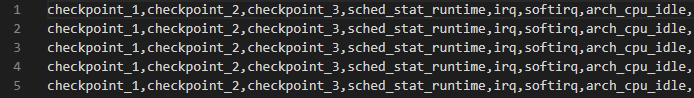
\includegraphics[width=\textwidth]{photos/name.png}
    \caption{Arquivo \textit{name}}
    \label{grafico:softirq}
\end{figure}

\begin{figure}[!htb]
    \centering
    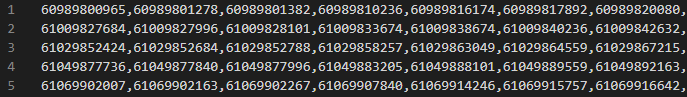
\includegraphics[width=\textwidth]{photos/ktime.png}
    \caption{Arquivo \textit{ktime\_mono\_fast}}
    \label{grafico:softirq}
\end{figure}


O repositório do INTSight fornece um script R que mescla esses arquivos em um único arquivo de saída usando as seguintes informações: \textit{position} (posição do item no teste), \textit{run} (número do teste na sequência), \textit{name} (evento que acionou a medição), \textit{ktime\_mono\_fast} (valor do contador). Apesar da disponibilidade desse script, o processamento de dados se mostrou lento, pois este código trata todos os dados na memória até que o resultado final esteja pronto para salvar em disco. Como o volume de dados foi muito grandes para o computador utilizado, com 12 GB de memória RAM, foi necessário utilizar o disco como memória auxiliar, isto tornou o tratamento dos dados lento. Portanto, a lógica do script disponibilizado pelo INTSight foi refeito utilizando a linguagem Python, mas ao tratar cada medição salvava imediatamente o resultado em um arquivo CSV, reduzindo o tempo para tratar cada sequência de teste de aproximadamente 2 horas para aproximadamente 20 minutos, no computador utilizado. Para consolidar os resultados das 18 sequências, gerando dados que serviram para montar as tabelas e gráficos comparativos utilizados nesse trabalho, foi escrito um script Python usando o Apache Spark, um framework para tratar grandes massas de dados \cite{Spark2009}, que abstraiu parte da lógica, tornando o script mais simples. Esse script também filtra os dados úteis, pois o INTSight pode salvar valores zero, devido a limitações com \textit{ktime\_mono\_fast}. Estas ocorrências são raras, menos de 1\% das medições, e devido a quantidade de medições realizadas por sequência de testes, 50.000 neste trabalho, a perda de algumas medições não afeta a análise realizada. 

\section{Visão global}

Para identificar as sequências de teste, um padrão de siglas foi adotado com base na versão do kernel, o tipo de mecanismo de interrupção e o indicador de carga do sistema. A primeira letra indica a versão do kernel: R para a versão padrão do Raspberry e P para a versão com o Preempt-RT. A segunda letra indica o mecanismo de interrupção testado: S para Softirq, T para Tasklet e W para Workqueue. A terceira letra indica a carga no processador: 0 thread, 1 thread ou M para 256 threads. Por exemplo, a sequência de teste do kernel padrão do Raspberry Pi, com o mecanismo Softirq e sistema com 0 thread de carga, tem a abreviação RS0. A sequência de teste do Preempt-RT, com o mecanismo de Workqueue e o sistema com 256 threads de carga, têm o acrônimo PWM.

Na tabela \ref{table:rpi}, encontra-se uma visão resumida da latência de ativação de todos os testes realizados com o kernel padrão e na tabela \ref{table:prt}, temos uma visão resumida da latência de ativação dos testes executados com Preempt-RT. Os percentis indicam de que aquela porcentagem das medições tiveram uma latência inferior ou igual ao valor na tabela.

\begin{table}[!htb]
\tiny
\centering
\begin{center}
\begin{tabular}{|c|r|r|r|r|r|r|r|r|r|}
\toprule
Percentil &    RS0 &     RS1 &    RSM &    RT0 &    RT1 &    RTM &    RW0 &     RW1 &      RWM \\
\midrule
    min &    \SI{833}{ns} &    \SI{365} {ns} &   \SI{ 781}{ns} &   \SI{ 625}{ns} &   \SI{ 938}{ns} &  \SI{  573} {ns}&  \SI{ 7604} {ns}&   \SI{ 5730} {ns}&    \SI{ 5156} {ns}\\
    25\% &   \SI{1041}{ns} &   \SI{937} {ns} &   \SI{ 937}{ns} &   \SI{1145}{ns} &   \SI{1145}{ns} &  \SI{ 1146} {ns}&  \SI{ 8021} {ns}&   \SI{ 8073} {ns}&    \SI{ 8750} {ns}\\
    50\% &   \SI{1042}{ns} &   \SI{938} {ns} &   \SI{ 938}{ns} &   \SI{1146}{ns} &   \SI{1146}{ns} &  \SI{ 1146} {ns}&  \SI{ 8124} {ns}&   \SI{ 8177} {ns}&    \SI{ 8854} {ns}\\
    75\% &   \SI{1094}{ns} &   \SI{990} {ns} &   \SI{ 990}{ns} &   \SI{1198}{ns} &   \SI{1198}{ns} &  \SI{ 1250} {ns}&  \SI{ 8229} {ns}&   \SI{ 8802} {ns}&    \SI{ 8958} {ns}\\
    90\% &   \SI{1146}{ns} &   \SI{1094}{ns} &   \SI{1042}{ns} &   \SI{1302}{ns} &   \SI{1302}{ns} &  \SI{ 1406} {ns}&  \SI{ 8489} {ns}&   \SI{ 9011} {ns}&    \SI{ 9218} {ns}\\
    99\% &   \SI{6041}{ns} &   \SI{5677}{ns} &   \SI{5937}{ns} &   \SI{6250}{ns} &   \SI{6251}{ns} &  \SI{ 6198} {ns}&  \SI{16666} {ns}&   \SI{18021} {ns}&    \SI{18282} {ns}\\
  99.9\% &   \SI{6927}{ns} &   \SI{6406}{ns} &   \SI{7187}{ns} &   \SI{7188}{ns} &   \SI{8073}{ns} &  \SI{10677} {ns}&  \SI{30520} {ns}&   \SI{27917} {ns}&    \SI{25052} {ns}\\
    \textbf{max} &  \textbf{\SI{15156}{ns}} &  \textbf{\SI{20365}{ns}} &  \textbf{\SI{19375}{ns}} &  \textbf{\SI{34998}{ns}} &  \textbf{\SI{25834}{ns}} &  \textbf{\SI{45260}{ns}} &  \textbf{\SI{84635}{ns}} &  \textbf{\SI{983798}{ns}} &  \textbf{\SI{4153458}{ns}} \\
\bottomrule
\end{tabular}
\end{center}
\caption{Principais dados das medidas do kernel padrão em nanossegundos}
\label{table:rpi}
\end{table}

\begin{table}[!htb]
\tiny
\centering
\begin{center}
\begin{tabular}{|c|r|r|r|r|r|r|r|r|r|}
\toprule
Percentil &    PS0 &    PS1 &    PSM &    PT0 &    PT1 &    PTM &    PW0 &     PW1 &    PWM \\
\midrule
  min  &   \SI{1197}{ns} &   \SI{1146}{ns} &   \SI{1197}{ns} &   \SI{1614}{ns} &   \SI{1563}{ns} &   \SI{1614}{ns} &  \SI{11563}{ns} &  \SI{11562}{ns} &  \SI{11562}{ns} \\
  25\% &   \SI{1406}{ns} &   \SI{1406}{ns} &   \SI{1406}{ns} &   \SI{1823}{ns} &   \SI{1823}{ns} &   \SI{1823}{ns} &  \SI{12084}{ns} &  \SI{12031}{ns} &  \SI{12083}{ns} \\
  50\% &   \SI{1407}{ns} &   \SI{1407}{ns} &   \SI{1458}{ns} &   \SI{1875}{ns} &   \SI{1875}{ns} &   \SI{1875}{ns} &  \SI{12239}{ns} &  \SI{12135}{ns} &  \SI{12187}{ns} \\
  75\% &   \SI{1459}{ns} &   \SI{1458}{ns} &   \SI{1459}{ns} &   \SI{1927}{ns} &   \SI{1927}{ns} &   \SI{1875}{ns} &  \SI{12396}{ns} &  \SI{12291}{ns} &  \SI{12344}{ns} \\
  90\% &   \SI{1510}{ns} &   \SI{1510}{ns} &   \SI{1510}{ns} &   \SI{1980}{ns} &   \SI{1979}{ns} &   \SI{1927}{ns} &  \SI{12761}{ns} &  \SI{12605}{ns} &  \SI{12656}{ns} \\
  99\% &   \SI{1979}{ns} &   \SI{1823}{ns} &   \SI{1979}{ns} &   \SI{2447}{ns} &   \SI{3073}{ns} &   \SI{3125}{ns} &  \SI{21928}{ns} &  \SI{20313}{ns} &  \SI{19323}{ns} \\
99.9\% &   \SI{4896}{ns} &   \SI{4062}{ns} &   \SI{4844}{ns} &   \SI{5364}{ns} &   \SI{5781}{ns} &   \SI{5468}{ns} &  \SI{40677}{ns} &  \SI{46146}{ns} &  \SI{39843}{ns} \\
\textbf{max} &  \textbf{\SI{18698}{ns}} &  \textbf{\SI{17656}{ns}} &  \textbf{\SI{17657}{ns}} &  \textbf{\SI{17343}{ns}} &  \textbf{\SI{16979}{ns}} &  \textbf{\SI{17865}{ns}} &  \textbf{\SI{80526}{ns}} &  \textbf{\SI{73854}{ns}} &  \textbf{\SI{86198}{ns}} \\
\bottomrule
\end{tabular}
\end{center}
\caption{Principais dados das medidas do Preempt-RT em nanossegundos}
\label{table:prt}
\end{table}

Podemos ver na tabela \ref{table:rpi} que no kernel padrão, a carga no sistema não influencia significativamente a latência dos mecanismos Softirq e Tasklet. Esses mecanismos são tratados no modo kernel e espera-se que a carga do sistema dos aplicativos no modo usuário não afete realmente esse tratamento. No entanto, para o mecanismo de Workqueue, tratado por threads dedicados e sujeito ao escalonador do sistema operacional, o aumento na carga do sistema faz com que a latência do pior caso aumente significativamente.

Examinando o Preempt-RT através da tabela \ref{table:prt}, vemos que a carga do sistema também não influencia a latência dos mecanismos Softirq e de Tasklet, como no kernel padrão. No entanto, diferentemente do kernel padrão, no mecanismo Workqueue, a latência também não muda significativamente devido à carga do sistema. Isso torna o Preempt-RT muito mais previsível, independentemente da carga aplicada pelos processos do usuário.

\section{Análise comparativa detalhada}

Ao analisar sistemas de tempo real, o interesse é como o sistema poderá responder dentro de um limite de tempo na pior das hipóteses. Aqui vamos comparar a latência entre os kernels e como eles se comportam em seus extremos. Os gráficos nas seções a seguir mostram os valores de latência nos percentis de 90\% a 99,9\%. O valor máximo foi omitido da visualização, pois esses são picos muito distantes do valor do percentil 99,9\%, especialmente para o kernel padrão, dificultando a análise visual do comportamento do kernel. A análise do pior caso é feita separadamente.

\subsection{Softirq}

No gráfico \ref{grafico:softirq}, podemos ver como os dois kernels se comportam no tipo de interrupção Softirq. O Preempt-RT tem uma latência mais alta nos casos médios que permanecem até aproximadamente os percentis entre 94,5\% e 97,5\%. Nesse intervalo, a latência padrão do kernel começa a aumentar, enquanto o Preempt-RT permanece estável até o percentil 98,5\%.

\begin{figure}[!htb]
    \centering
    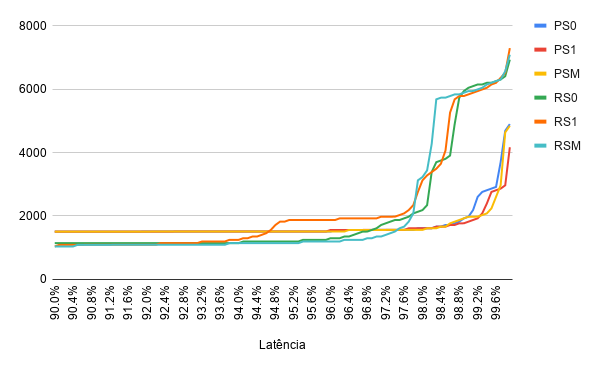
\includegraphics[width=\textwidth]{graficos/softirq.png}
    \caption{Latência com Softirq em nanossegundos}
    \label{grafico:softirq}
\end{figure}

\begin{table}[!htb]
    \centering
    \begin{center}
        \begin{tabular}{|c|c|c|c|c|c|c|}
            \toprule
                Latência & PS0 &    PS1 &    PSM &    RS0 &     RS1 &    RSM \\
            \midrule
                máx & 18698 &  17656 &  17657 & 15156 &  20365 &  19375 \\
            \bottomrule
        \end{tabular}
    \end{center}
    \caption{Latência máxima para o Softirq}
    \label{table:max-softirq}
\end{table}

Para o pior caso de cada sequência de teste, temos a tabela \ref{table:max-softirq}. Nos casos com sistema ocioso, o Preempt-RT teve uma latência pior que o kernel padrão para o pior caso. Com a carga do sistema com 1 thread, o Preempt-RT teve uma leve redução no pior caso, enquanto o kernel padrão teve um aumento na latência. Com o sistema sobrecarregado, os dois kernels apresentaram valores próximos ao nível do sistema com carga de 1 thread.

Nos gráficos de dispersão para medições do Softirq no kernel padrão \ref{grafico:r-softirq} e Preempt-RT \ref{grafico:p-softirq}, podemos observar que existem muitos valores em uma faixa mais baixa e uma faixa menor com valores mais altos. O kernel padrão possui valores médios mais baixos para o intervalo inferior, mas possui um intervalo superior com valores mais altos. No Preempt-RT, a faixa superior está muito mais próxima da faixa inferior.

\begin{figure}[!htb]
    \centering
    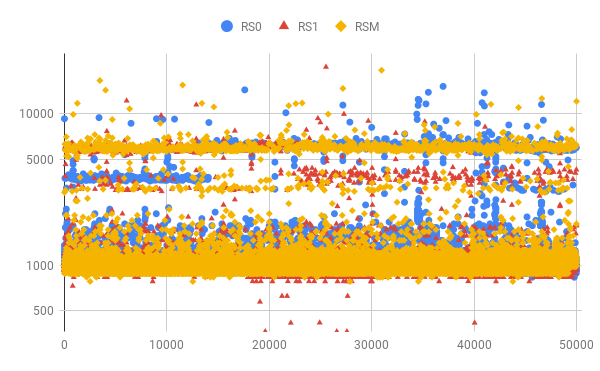
\includegraphics[width=\textwidth]{graficos/rs-scatter.png}
    \caption{Latência da sequência de testes com Softirq no kernel padrão}
    \label{grafico:r-softirq}
\end{figure}

\begin{figure}[!htb]
    \centering
    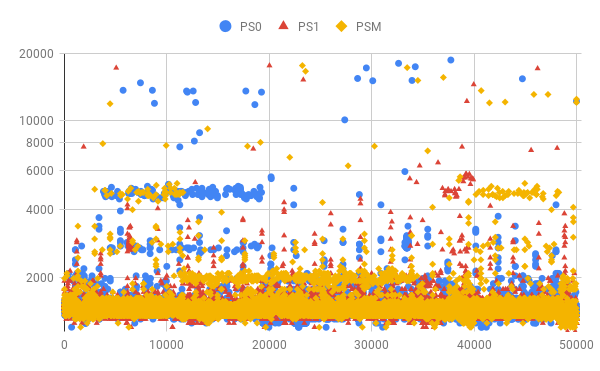
\includegraphics[width=\textwidth]{graficos/ps-scatter.png}
    \caption{Latência da sequência de testes com Softirq no Preempt-RT}
    \label{grafico:p-softirq}
\end{figure}

\subsection{Tasklet}

Para o tipo de interrupção Tasklet, os dois kernels se comportam de maneira semelhante ao Softirq, mas com uma latência um pouco maior, como podemos ver no gráfico \ref{grafico:tasklet}. O kernel padrão tem melhores latências até aproximadamente 95\% quando possui carga no sistema ou em torno de 98\% quando o sistema está ociosa. Também na faixa de 98\% é quando o Preempt-RT começa a aumentar a latência.

\begin{figure}[!htb]
    \centering
    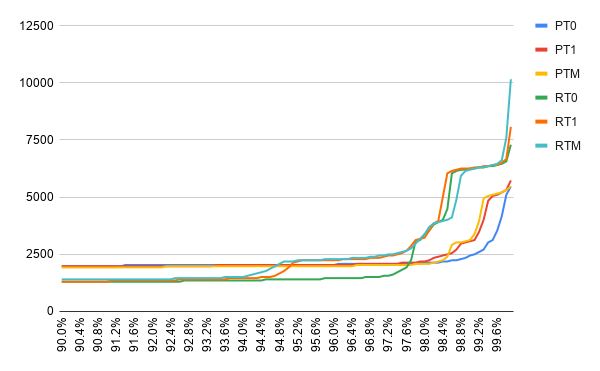
\includegraphics[width=\textwidth]{graficos/tasklet.png}
    \caption{Latência com Tasklet em nanossegundos}
    \label{grafico:tasklet}
\end{figure}

\begin{table}[!htb]
    \centering
    \begin{center}
        \begin{tabular}{|r|r|r|r|r|r|}
            \toprule
                PT0 &    PT1 &    PTM &    RT0 &     RT1 &    RTM \\
            \midrule
                17343 &  16979 &  17865 & 34998 &  25834 &  45260  \\
            \bottomrule
        \end{tabular}
    \end{center}
    \caption{Latência máxima para o Tasklet}
    \label{table:max-tasklet}
\end{table}

Na tabela \ref{table:max-tasklet} temos os valores de pior caso para os testes com o Tasklet. Podemos ver que o Preempt-RT quase não sofreu influência com o nível de carga do sistema. No kernel padrão, há uma ligeira variação entre os valores, dependendo da carga imposta, mas ainda uma variação dentro de uma faixa não muito ampla.

Diferentemente do Softirq, a latência máxima do Tasklet no Preempt-RT é muito menor do que no kernel padrão. O Preempt-RT possui uma latência máxima que é quase metade da latência do kernel padrão.

A dispersão do Tasklet é semelhante ao Softirq, como visto nos gráficos \ref{grafico:r-tasklet} e \ref{grafico:p-tasklet}. No kernel padrão, o número de valores que divergem do intervalo superior não parece ser maior que no Preempt-RT, mas os valores são mais distantes da faixa comum.

\begin{figure}[!htb]
    \centering
    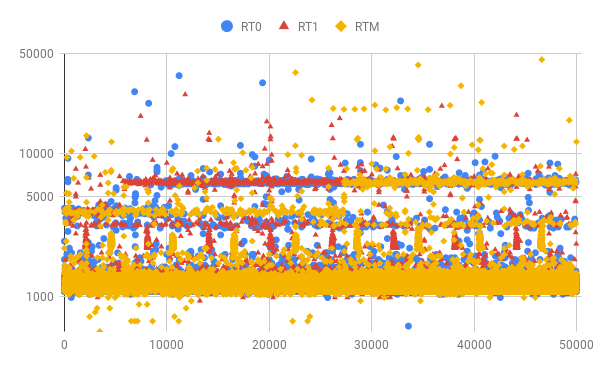
\includegraphics[width=\textwidth]{graficos/rt-scatter.png}
    \caption{Latência da sequência de testes com Tasklet no kernel padrão}
    \label{grafico:r-tasklet}
\end{figure}

\begin{figure}[!htb]
    \centering
    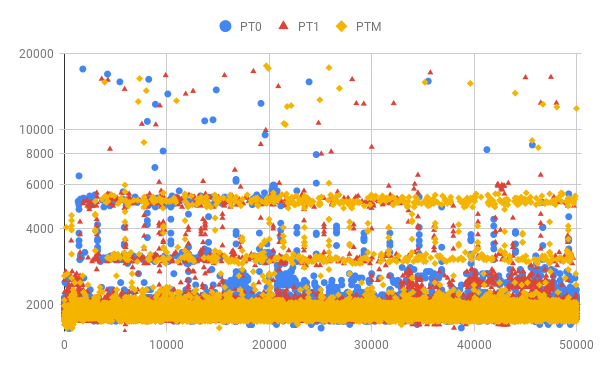
\includegraphics[width=\textwidth]{graficos/pt-scatter.png}
    \caption{Latência da sequência de testes com Tasklet no Preempt-RT}
    \label{grafico:p-tasklet}
\end{figure}

\subsection{Workqueue}

No tipo de interrupção Workqueue, as diferenças são sutis se a latência máxima não for levada em consideração e a figura \ref{grafico:workqueue} mostra isso bem. Por outro lado, se formos analisar apenas a latência máxima, a diferença entre os kernels é muito alta, como podemos ver na tabela \ref{table:max-workqueue}.

\begin{figure}[!htb]
    \centering
    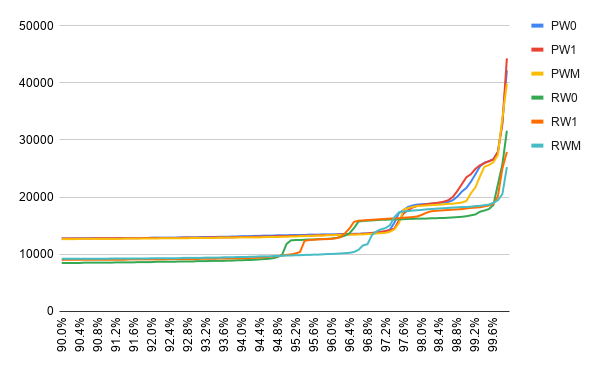
\includegraphics[width=\textwidth]{graficos/workqueue.png}
    \caption{Latência com Workqueue em nanossegundos}
    \label{grafico:workqueue}
\end{figure}

\begin{table}[!htb]
    \centering
    \begin{center}
        \begin{tabular}{|r|r|r|r|r|r|}
            \toprule
                PW0 &    PS1 &    PWM &    RW0 &     RW1 &    RWM \\
            \midrule
                80526 &  73854 &  86198 & 84635 &  983798 &  4153458 \\
            \bottomrule
        \end{tabular}
    \end{center}
    \caption{Latência máxima para o Workqueue}
    \label{table:max-workqueue}
\end{table}

Ambos os kernels têm uma latência semelhante quando não há carga no sistema, mas com 1 thread de carga, o kernel padrão tem uma latência máxima mais de 10 vezes maior em comparação com a situação com o sistema ocioso. No Preempt-RT, há uma ligeira queda no tempo máximo.

Ao considerar um sistema sobrecarregado, a latência do Preempt-RT aumentou um pouco, mas permaneceu próximo aos valores do sistema sem carga. Já o kernel padrão, teve uma latência quase 50 vezes maior com sobrecarga do sistema em comparação com o cenário ocioso.

No gráfico \ref{grafico:r-workqueue}, podemos ver a dispersão das medições no Workqueue com as diferentes cargas. Podemos observar que, quando o sistema está sobrecarregado, a ocorrência de pontos fora da média ocorre mais de uma vez e com valores muito acima da média, tornando a latência não determinística.

\begin{figure}[!htb]
    \centering
    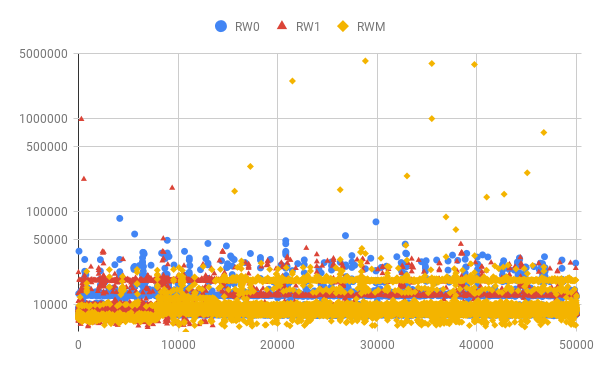
\includegraphics[width=\textwidth]{graficos/rw-scatter.png}
    \caption{Latência da sequência de testes com Workqueue no kernel padrão}
    \label{grafico:r-workqueue}
\end{figure}

Para o Preempt-RT, a dispersão é menor, como podemos ver no gráfico \ref{grafico:p-workqueue}. Os piores casos estão próximos um do outro e não tão longe da média. Não há valores que se afastem muito de um conjunto de valores que representa bem o grupo.

\begin{figure}[!htb]
    \centering
    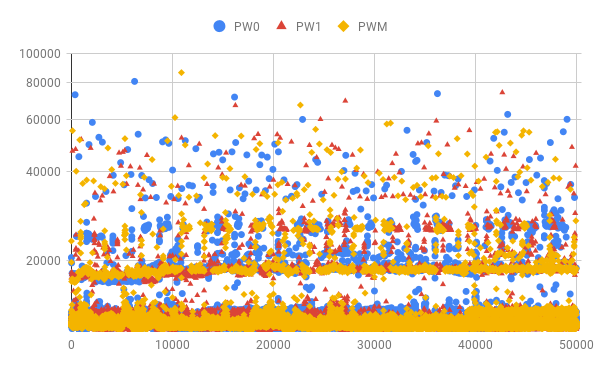
\includegraphics[width=\textwidth]{graficos/pw-scatter.png}
    \caption{Latência da sequência de testes com Workqueue no Preempt-RT}
    \label{grafico:p-workqueue}
\end{figure}

\section{Discussões sobre os resultados}

A implementação de um Softirq envolve a compilação de todo o kernel e não possui diferença significativa entre o kernel padrão e o Preempt-RT. Se for realmente necessário implementar a interrupção como Softirq, não há necessidade de usar o Preempt-RT, pois há um custo associado ao ter o kernel totalmente preemptivo.

Ao optar por implementar a interrupção como Tasklet em um módulo do kernel, há diferenças na latência entre o kernel padrão e o Preempt-RT, sendo o Preempt-RT mais responsivo. No entanto, a variação na latência padrão do kernel com a carga do sistema não é tão grande. Se o pior caso medido for suficiente para atender às restrições de tempo do sistema, o kernel padrão poderá desempenhar o papel de sistema em tempo real sem onerar as demais tarefas.

Ao analisar o Workqueue, a diferença entre o kernel padrão e o Preempt-RT se torna evidente. Se a interrupção for implementada como Workqueue e for necessário um sistema que atenda às restrições de tempo, o Preempt-RT é a escolha a ser feita.

Levando em consideração os dados obtidos com as medições deste trabalho e tomando como exemplo um sistema que tenha uma tarefa periódica que precisa responder a cada \SI{200}{\micro\second}, o tempo que a aplicação terá disponível para efetuar os cálculos a depender dos mecanismos de tratamento de interrupção utilizados será:

\begin{itemize}
    \item com o mecanismo Softirq, a aplicação terá que efetuar seus cálculos em até \SI{179}{\micro\second} na versão padrão e em até \SI{181}{\micro\second} na versão com o Preempt-RT;
    \item com o mecanismo Tasklet, a aplicação terá que efetuar seus cálculos em até \SI{154}{\micro\second} na versão padrão e em até \SI{172}{\micro\second} na versão com o Preempt-RT;
    \item com o mecanismo Workqueue, a aplicação não tem qualquer garantia temporal na versão padrão e tem até \SI{113}{\micro\second} na versão com o Preempt-RT;
\end{itemize}

Estes dados ajudam a decidir se uma aplicação pode ser implementada ou não no Raspberry Pi e quais os mecanismos serão necessários para se atingir as garantias temporais.